\begin{table*}
  \centering
  \caption{Target text-based Captcha schemes used in our experiment}
  \label{tab: captcha_show}
  \small
  \begin{tabular}{|c|c|c|c|c|}
    \hline
     &  &  & \multicolumn{2}{|c|}{Security Features} \\
     \cline{4-5}
    \multirow{-2}{*}{Scheme} & \multirow{-2}{*}{Website} & \multirow{-2}{*}{Sample} & Anti-segmentation Features & Anti-recognition Features \\
    \hline
    Google & google.com & \tabincell{c}{
\includegraphics[width=0.1\textwidth]{fig/experiment_captchas/google1.jpg} 
\includegraphics[width=0.1\textwidth]{fig/experiment_captchas/google2.jpg}} & \tabincell{c}{ Overlapping characters, \\ only Enligh letters used} & \tabincell{c}{Varied font size, color, \\ rotating, disortion and waving used} \\
    \hline
    Baidu & baidu.com & \tabincell{c}{
\includegraphics[width=0.1\textwidth]{fig/experiment_captchas/baidu3.jpg} 
\includegraphics[width=0.1\textwidth]{fig/experiment_captchas/baidu2.jpg}} & \tabincell{c}{Connecting Lines, overlapping, \\ only Enligh letters used} & \tabincell{c}{Both hollow and solid characters, \\ varied font size, color, \\ rotating, disortion and waving used} \\
    \hline
    Alipay & alipay.com & \tabincell{c}{
\includegraphics[width=0.1\textwidth]{fig/experiment_captchas/alipay1.jpg} 
\includegraphics[width=0.1\textwidth]{fig/experiment_captchas/alipay2.jpg}} & \tabincell{c}{Overlapping characters used} & \tabincell{c}{Both English letters and \\ Arabic numerals, \\ rotating and distortion used} \\
    \hline
     Wikipedia& wikipedia.org & \tabincell{c}{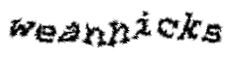
\includegraphics[width=0.1\textwidth]{fig/experiment_captchas/wikipedia1.png} 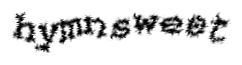
\includegraphics[width=0.1\textwidth]{fig/experiment_captchas/wikipedia2.png}} & \tabincell{c}{Only English letters used} & \tabincell{c}{Character rotating, \\ distortion and waving} \\
     \hline
     Sohu& sohu.org & \tabincell{c}{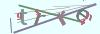
\includegraphics[width=0.1\textwidth]{fig/experiment_captchas/sohu1.jpg} 
\includegraphics[width=0.1\textwidth]{fig/experiment_captchas/sohu2.jpg}} & \tabincell{c}{Complex background, \\ connection lines, \\and overlapping used} & \tabincell{c}{varied font size, color \\ and character rotating} \\
    \hline
    NetEase & 163.com & \tabincell{c}{
\includegraphics[width=0.1\textwidth]{fig/experiment_captchas/netease1.jpg} 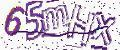
\includegraphics[width=0.1\textwidth]{fig/experiment_captchas/netease2.jpg}} & \tabincell{c}{Complex background, \\ connecting lines} & \tabincell{c}{Both hallow and solid characters, \\ varied rotating angles used} \\
    \hline
    VIPSHOP & vip.com & \tabincell{c}{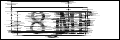
\includegraphics[width=0.1\textwidth]{fig/experiment_captchas/vipshop1.jpg} 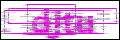
\includegraphics[width=0.1\textwidth]{fig/experiment_captchas/vipshop2.jpg}} & \tabincell{c}{Complex background, \\ overlapping characters} & \tabincell{c}{Both English letters \\ and Arabic numerals, \\ varied font colors used} \\
    \hline
     TOUP& tuniu.com & \tabincell{c}{ 
\includegraphics[width=0.1\textwidth]{fig/experiment_captchas/tuniu1.jpg} 
\includegraphics[width=0.1\textwidth]{fig/experiment_captchas/tuniu2.jpg}} & \tabincell{c}{Overlapping characters used} & \tabincell{c}{Both English letters \\ and Arabic numerals, \\ waving characters used} \\
    \hline
  \end{tabular}
\end{table*}

\section{Experimental Setup}
\subsection{Data Preparation and Collection}
The Captchas used in our evaluation are made up of both training data and testing data, and they come from two different sources. The training Captchas are synthesized by our Captcha generator (Section~\ref{section: Captcha_generator}) and the testing Captchas are collected from target websites using a traditional mining method written through a python script.

\noindent \textbf{Target Websites.} We select the target websites based on the following rules: (1) the Captchas of website combines at least one anti-segmentation and three anti-recognition features; (2) the website must have a large number of active users and (3) the target websites should cover as many industries as possible.
%(3) the testing Captchas are relatively easy to mine~\footnote{Some Captcha schemes, such as Tecent Captchas, are hard to mine as each Captcha image has a different URL.}.  
According to the three factors, we target 18 famous websites for preparing our data. These target websites can be classified into 5 categories: \emph{E-commerce site} (such as Ebay, Alipay, JD and Alipayexpress), \emph{Social Networks} (such as Live and Sina Microblog), \emph{Search Engine} (such as Google, Baidu, 360 and Bing), \emph{Portal sites} (such as Wikipedia, Sohu and Sina) and other sites (such as Yutube and Microsoft Office).
 Table~\ref{tab: captcha_show} presents some Captcha schemes of target websites and their security features.
%\textcolor{red}{5 famous websites for preparing our data: Baidu, Alipay, NetEase, VIPSHOP and TOUP}.


\noindent \textbf{Synthesize Training Captchas.} To ensure the synthesized Captcha as likely as the true one, we first manually analyze the traits of the true Captchas and aggregates these traits to a feature tuple as described in Section~\ref{section: Captcha_generator}. According to the feature tuple, a large number of training Captchas can be synthesized by our generator. In our experiment, we totally synthesized 15 kinds of Captchas come from the target websites. For each website, we mined 20000 Captchas to be used for training process.

\noindent \textbf{Mine Testing Captchas.} The testing Captchas used in our evalustion are automatically mined from the target websites using a python script. For each target website, we apply 2000 Captchas to test the efficiency of our attacking system.  We recruited nine participators from our institution to manually mark the labels of the mined Captchas. To decrease the marking error rate, the nine participator are divided into three groups and each group has three people. We choose these Captcha which two participators mark the correct tags of the Captchas at the same time as the testing data.

\subsection{Implementation} 
Our prototyped attacking system built upon a variant of \emph{Pix2Pix} framework~\cite{Pix2PixCode} in Tensorflow. The developed software ran on an ordinary
server with a 3.2-GHz Inter Xeon CPU with 100-GB RAM and a TITAN Xp GPU. The operating system is Ubuntu 16.04.

%\subsection{Captchas Show}
